


\documentclass[10pt, handout]{beamer}
\setbeamertemplate{navigation symbols}{}
\usefonttheme{serif} 
\usepackage{amsmath}
\usepackage{amssymb}
\usepackage{graphicx}
\usepackage{cite}
\usepackage{color} 
\usepackage{setspace}
\usepackage{hyperref}

\newcommand{\xx}{{\bf{x}}}

\begin{document}
\title{Machine Learning I Lecture V:\\ Linear Regression Revisited}   
\author{Jakob H Macke\\ Max Planck Institute for Biological Cybernetics\\ Bernstein Center for Computational Neuroscience} 
\date{XY.XY.2012} 

\frame{\titlepage} 

%\frame{\frametitle{Today: Back to basics of probability theory}} 


\frame{\frametitle{Plan for today}\tableofcontents} 


\section{Linear regression revisited}
\frame[shrink=2]{\frametitle{Linear regression can be considered as  maximum likelihood estimation in a Gaussian model.}
\begin{itemize}
\item Suppose that we have data $D=\{(\xx_1, t_1), \ldots, (\xx_N, t_N) \}$
\item We assume that the data can be modelled by some function $t_n \approx y(x, \omega)+ \epsilon$, where $\epsilon$ models additive noise.
\item \pause We assume that noise is independent, identically distributed and Gaussian: 
\begin{align}
\epsilon &\sim \mathcal{N}(0,\beta^{-1})\\
t|\xx, \omega, \beta &\sim \mathcal{N}(y(\xx,\omega), \beta^{-1})
\end{align}
\end{itemize}
\centering
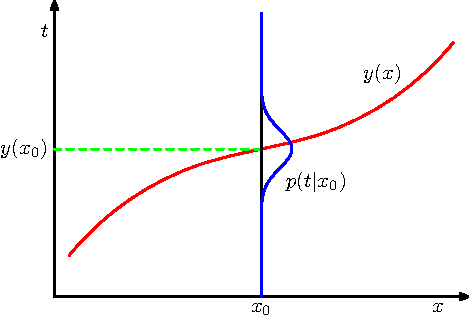
\includegraphics[width=.5\textwidth]{Figure128.pdf}\\
\tiny Bishop PRML Figure 1.28 
}


\frame{\frametitle{Linear regression can be considered as  maximum likelihood estimation in a Gaussian model.}

\begin{itemize}
\item We consider a linear model $y(\xx,\omega)= \omega^\top \xx$
\item ~[On board: Likelihood, Maximum Likelihood Solution, Predictive distribution from MLE]\\
\vspace{3cm}
\item \pause For a Bayesian treatment, we need priors.
\end{itemize}
}
%Note: 



\frame{\frametitle{We use a multivariate Gaussian as a prior on the parameters $\omega$.}
\begin{align}
\omega_i &\sim \mathcal{N}(0,\alpha^{-1})\\
p(\omega| \alpha) &= \prod_{i=1}^M  \sqrt{\frac{\alpha}{{2\pi}}}\exp\left( -\frac{\alpha}{2}  {\omega_i^2}\right)\\
&%\pause
 =\left(\frac{\alpha}{2\pi}\right)^{M/2} \exp \left(-\frac{\alpha}{2} \omega^\top \omega  \right)
\end{align}
\pause
\begin{itemize} %\pause
\item Finding the maximum-a-posteriori of $\omega$: [on board]
\end{itemize}

}

\frame{\frametitle{If you are smart about choosing good basis functions ('features'), linear regression can get you pretty far.}
\begin{itemize}
\item If we use nonlinear basis functions $\phi(x)$, can model nonlinear relationships with $y(\omega, \xx)= \omega^\top \phi(x)$.
\item Polynomial regression: $\phi(x)=(1,x,x^2,x^3)$
\item 'Gaussian bumps': $\phi_i(x)= \exp\left((x-s_i)^2/\sigma_i^2 \right)$
\item Sigmoids $\phi_i(x)=1/(1+\exp(-x-s_i))$
\item \pause 'Kernel methods' are essentially linear algorithms which take one basis function per data-point.
\item Predictive Mean [on board]
\end{itemize}
\centering
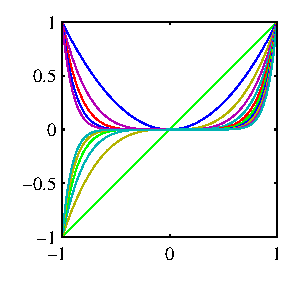
\includegraphics[width=.3\textwidth]{Figure31a.pdf}
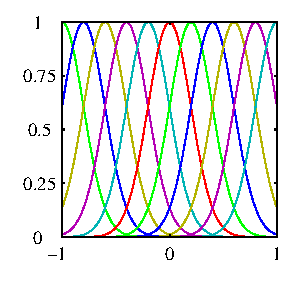
\includegraphics[width=.3\textwidth]{Figure31b.pdf}
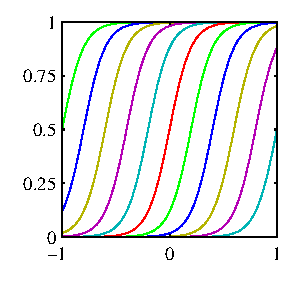
\includegraphics[width=.3\textwidth]{Figure31c.pdf}
\tiny Bishop PRML Figures 3.1a-c
}




\section{Bayesian linear regression}


\frame{\frametitle{Bayesian linear regression takes into account our uncertainty about parameters.}

\begin{itemize}
\item Posterior distribution is Gaussian $\rightarrow$ Posterior mean and MAP coincide!
\item \pause However, neither the MLE nor the MAP solution take into account that we have (posterior) uncertainty about the parameters
\end{itemize}
\centering ~

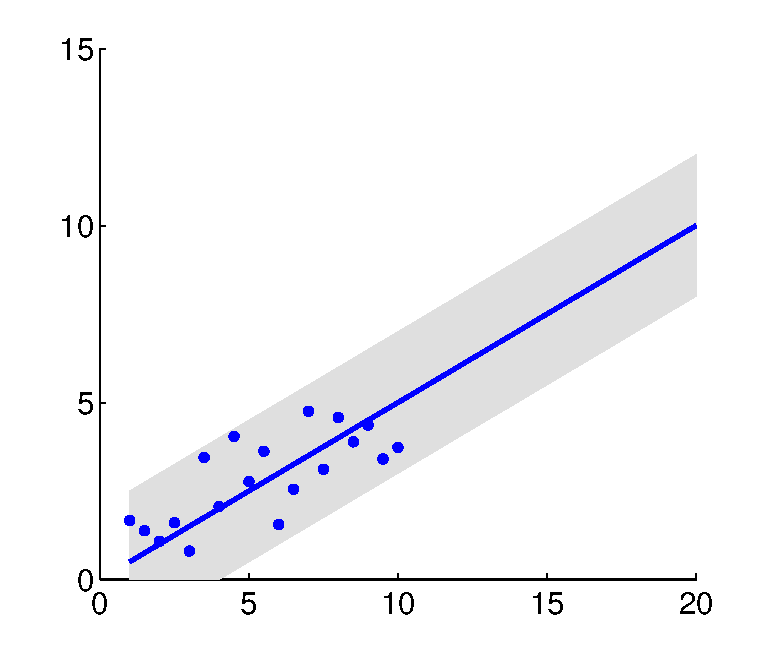
\includegraphics[width=.45\textwidth]{./matlab/LinReg.pdf}
\pause
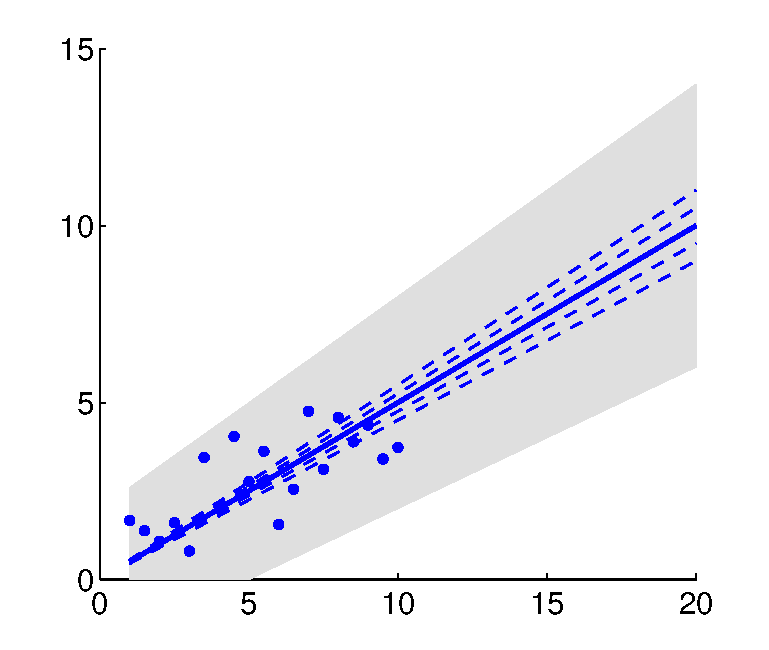
\includegraphics[width=.45\textwidth]{./matlab/LinRegBayes.pdf}
}


\frame{\frametitle{Illustration: Climate prediction [by Carl Rasmussen, University of Cambridge, using Gaussian Processes]}

%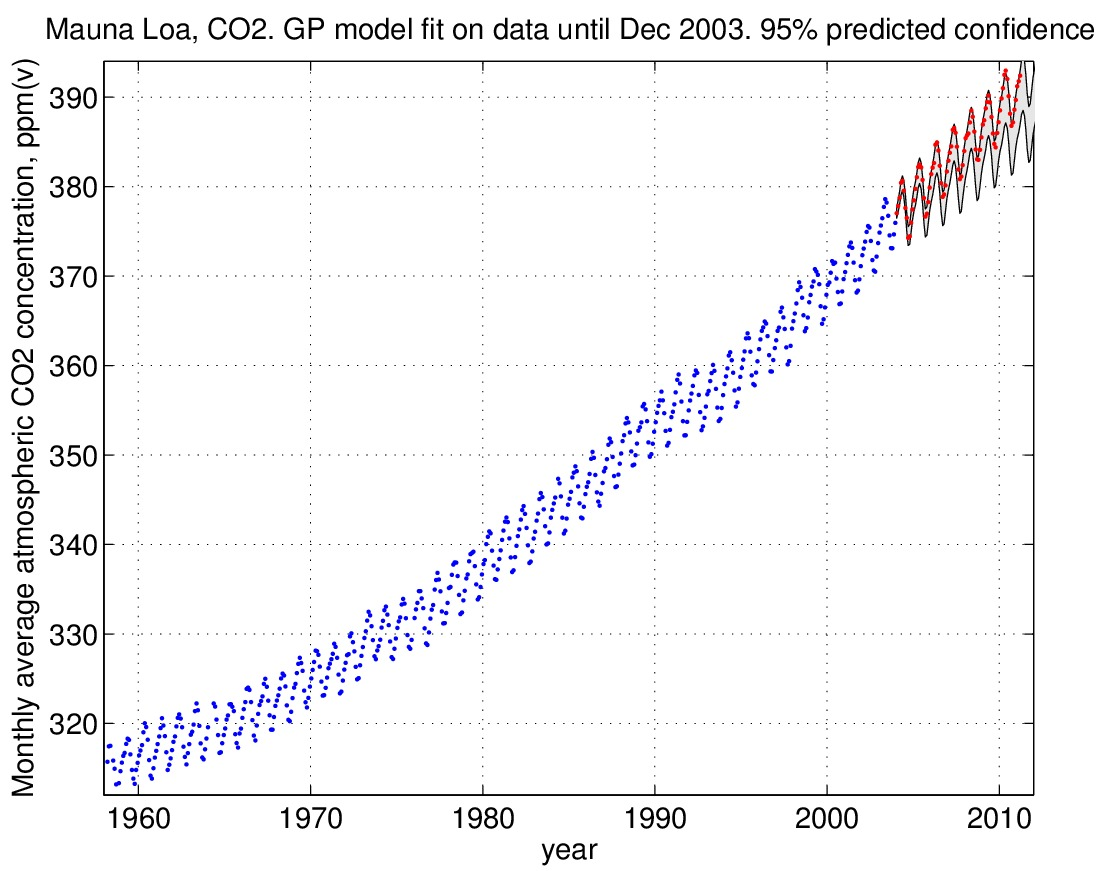
\includegraphics[width=.49\textwidth]{Rasmussen1}
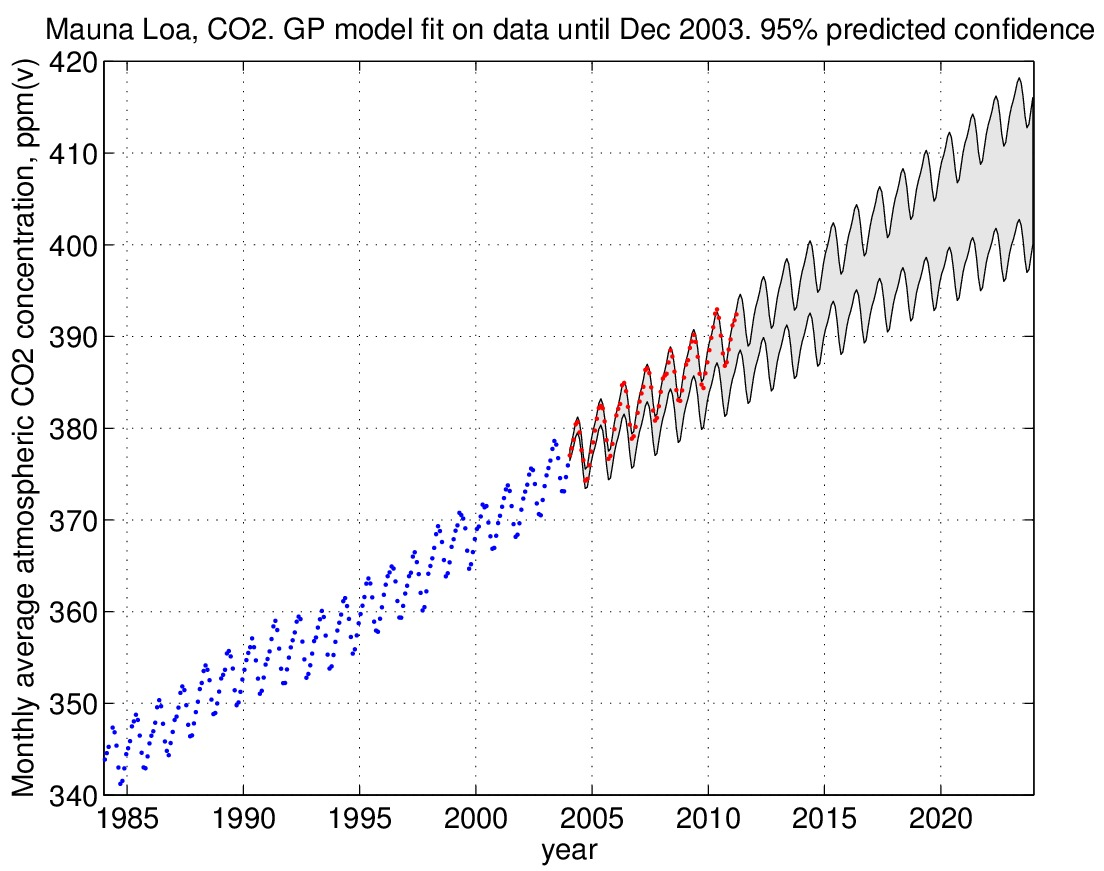
\includegraphics[width=.9\textwidth]{Rasmussen2}

}


\frame{\frametitle{Bayesian regression illustrated: The more data we observe, the more constrained the parameters are.}

%\vspace{-.1cm}
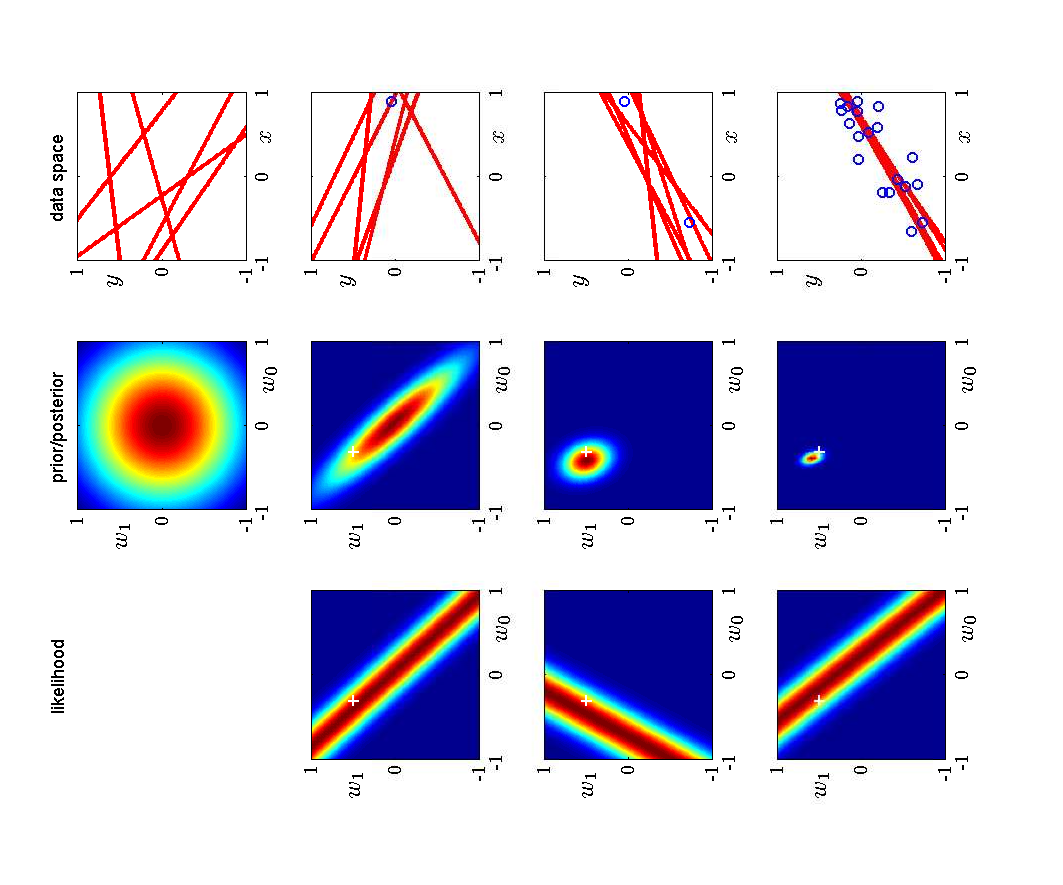
\includegraphics[width=.8\textwidth]{Figure37.pdf}

\tiny Bishop PRML Figure 3.7
}


\frame{\frametitle{Calculating the predictive mean and variance for Bayesian regression}


%\begin{itemize}
Assume $\alpha$ and $\beta$ as given.\\ Posterior distribution: [derivation on board]
\pause
\begin{align}
\Sigma_{post}^{-1}&=\alpha \mathbf{I}+\beta \sum_i x_i x_i^\top\\
\mu_{post}&=\Sigma_{post} \beta \sum_i x_i t_i
\end{align}

%\end{itemize}
\pause
Predictive distribution: [derivation on board]
\pause
\begin{align}
E(t^*|D,x^*)&= \mu_{post}^\top x^* \\
\mbox{Var}(t^*|D,x^*)&=  1/\beta+ x^{*\top} \Sigma_{post} x^*
\end{align}
%\item 
\pause What if there are basis functions? [on board]
}


\section{Fully Bayesian linear regression}


\frame{\frametitle{But, where do we get $\alpha$ and $\beta$ from?}

\begin{itemize}
\item Bad news: Getting these makes things more complicated.
\item \pause Good news: This will not be on the exam (unless I take that back explicitly...). 
\item \pause 'Full' Bayesian inference: Integrate out $\alpha$, $\beta$. No closed form solution. Use (e.g.) variational inference.
\item \pause Practical solution: optimize $\alpha$ and $\beta$ by \alert{maximizing the evidence}, also known as \alert{marginal likelihood} or \alert{likelihood type 2}
\begin{align}
E&=\log P(\alpha, \beta|D)\\
&=\pause \log \int_\omega p(D|\omega,\beta) p(\omega|\alpha) p(\alpha,\beta)    d \omega\\
&=\pause \frac{M}{2}\log(\alpha)+\frac{N}{2}\log \beta-\mbox{M}(\mu_{post})+\frac{1}{2}|\Sigma_{post}|-\frac{N}{2} \log(2\pi) 
\end{align}
\item $\mu_{post}$ and $\Sigma_{post}$ are the posterior mean and covariance, and $\mbox{M}(\mu_{post})=\frac{\beta}{2}\sum_n (t_n-y(\mu_{post},\xx_n))^2+\frac{\alpha}{2} \mu_{post}\mu_{post}^\top$ is the quadratic cost function evalulated at the posterior mean (see Bishop 3.5 for details).
\end{itemize}



}
\frame{\frametitle{Optimization of the marginal likelihood is a Bayesian alternative to parameter-setting by cross-validation.
}

[on board] 
}



\frame{\frametitle{What we have not had time to cover:
}
\begin{itemize}
\item \alert{Non-Gaussian priors:} The most important non-Gaussian prior is the `Laplace prior' ('L1 regularization'), which leads to sparse MAP-solutions.
\item \alert{Non-Gaussian noise models:} If you know that your noise is not Gaussian but, say, Poisson, use 'generalized linear regression'. Some choices of noise models are more robust to outliers than the Gaussian. We will do one specific example of generalized linear regression in the last lecture.
\item \alert{Nonlinear regression models:} The most important Bayesian nonlinear regression technique is \emph{Gaussian process regression}. In a nutshell, GP regression is like linear regressions but the algorithm puts ne basis function at each data-point. To understand GP regression, you need to understand Gaussians.
\end{itemize}
}


\end{document}

\frame{\frametitle{Do you want a tutorial before the exam?} 
\begin{itemize}
\item As I added 1.5 Lectures on background in probability theory, we are behind schedule. 
\item Therefore, I cut out some material from the syllabus (nonlinear regression). This is not terrible, as this will apparently also be covered in Machine Learning II. 
\item In addition, the last lecture was supposed to be a tutorial, but will be a proper lecture now.
\item So, if you want a tutorial before the exam, we will have to organize it now. 
\end{itemize}

%I hope you appreciate that this is a service from me to you-- you will need proabbility theory in very many courses.
}




 



